We introduce the $10 \times 10$ gridworld Figure \ref{fig:gridworld1} which has the following features:-

\begin{enumerate}
\item The starting state is shown as $S$ in green color.
\item At any grid, only four discrete actions are possible, left, right, bottom, top.
\item The obstacles are shown in red colors. When an agent hits the obstacles, it stays in the state before attempting to transition.
\item The only difference between Domain \ref{fig:gridworld1} and Domain \ref{fig:gridworld2} is the position of the death state $S_t = D$. 
\item The terminal states are shown in orange. $D$ represents the state "death" with a negative reward of $R(S_t = D, A_t = a) = -60$ while $G$ represents the state "get well" with a time-varying reward of $R(S_t = G, A_t = a) = 60 - t$, $1\leq t \leq 60$. All the other transitions result in a reward of $0$.
\item Note, that the time $t$ is part of the representation of state as rewards are changing with time $t$.
\item The states are featurized by the function $\Phi: S \rightarrow R^{r+c}$, where $r$ is the number of rows and $c$ is the number of columns in the gridworld. So, $\Phi(s)$ is a function that maps states to vectors of features. We define $\Phi(s)$ such that for the state $s_{i,j}$, where $i$ is the row-index and $j$ is the column index in the grid, then $\Phi(s_{i,j})$ is the vector $v$ such that,
\begin{align*}
v_{k} &= 1 \text{, if k = i+j}\\
&= 0 \text{ otherwise,}
\end{align*}

and $k=1,\ldots,(r+c)$ is the index of the vector $v$.
\end{enumerate}

Next, we illustrate why these features where included in these gadget worlds and link up with our discussion on the complexities of the medical domain.

\begin{enumerate}
\item The state space is discrete and and the action space is also finite and  discrete. We wanted to keep the gadget worlds simple.
\item  Domain \ref{fig:gridworld2} is slightly more difficult than Doamin \ref{fig:gridworld1} as the path to "get well" state $S_t = G$ is more restricted in the former.
\item There is only substantial reward (positive/negative) at the end of the long episodes when the agent reaches the states either $S_t = G$ or $S_t = D$. This handles the long horizon problem.
\item Rewards are also adversarial as they are changing with time. Because of this, if the agent reaches the goal state at $t = 60$, it receives a reward of $0$. Moreover, the rewards are diminishing with time indicating, that the agent has to reach the terminal "get well" state quickly.
\item The partially observed environment is captured in how we are featurizing the states. Note that $\Phi(s_{2,3})$ will have the same embedding as $\Phi(s_{3,2})$. This follows from the idea that when feature representation of states are \textit{not} rich enough it result in a partially observed environment. 
\item The obstacles, (marked in red) forces the q-value function approximator not to generalize too well. These makes the simple environment slightly more difficult to be generalized well enough.
\end{enumerate}


\begin{figure}[!th]
\begin{center}
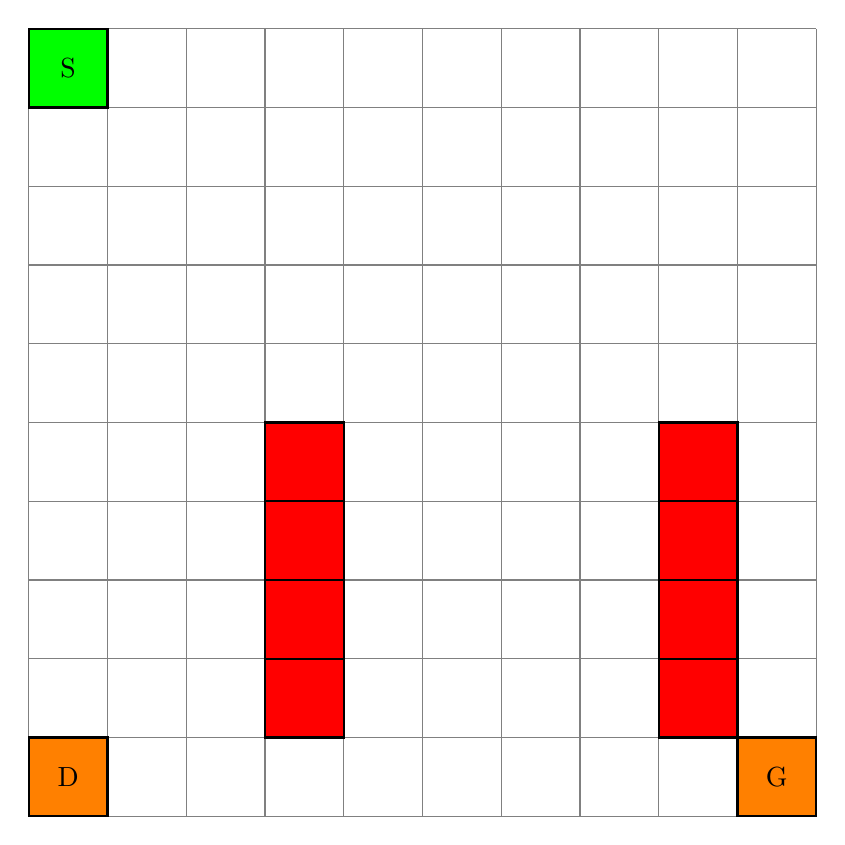
\begin{tikzpicture}
\draw[step=1.0 cm,color=gray] (0,0)grid (10,10);
% col, row
\node[rectangle,draw=black,thick, minimum size=1cm, fill=green] at (.5,9.5) {S};
\node[rectangle,draw=black,thick, minimum size=1cm, fill=red] at (3.5,1.5) {};
%\fill[red!10!white] (0,0) rectangle (1,1);
%\node[fill=green] at (8,8){};  
\node[rectangle,draw=black,thick, minimum size=1cm, fill=red] at (3.5,2.5) {};
\node[rectangle,draw=black,thick, minimum size=1cm, fill=red] at (3.5,3.5) {};
\node[rectangle,draw=black,thick, minimum size=1cm, fill=red] at (3.5,4.5) {};
\node[rectangle,draw=black,thick, minimum size=1cm, fill=red] at (8.5,1.5) {};
\node[rectangle,draw=black,thick, minimum size=1cm, fill=red] at (8.5,2.5) {};
\node[rectangle,draw=black,thick, minimum size=1cm, fill=red] at (8.5,3.5) {};
\node[rectangle,draw=black,thick, minimum size=1cm, fill=red] at (8.5,4.5) {};
\node[rectangle,draw=black,thick, minimum size=1cm, fill=orange] at (9.5,.5) {G};
\node[rectangle,draw=black,thick, minimum size=1cm, fill=orange] at (.5,.5) {D};
\end{tikzpicture}
\end{center}
\caption{Medical Domain 1 Grid World}
\label{fig:gridworld1}
\end{figure}


\begin{figure}[!th]
\begin{center}
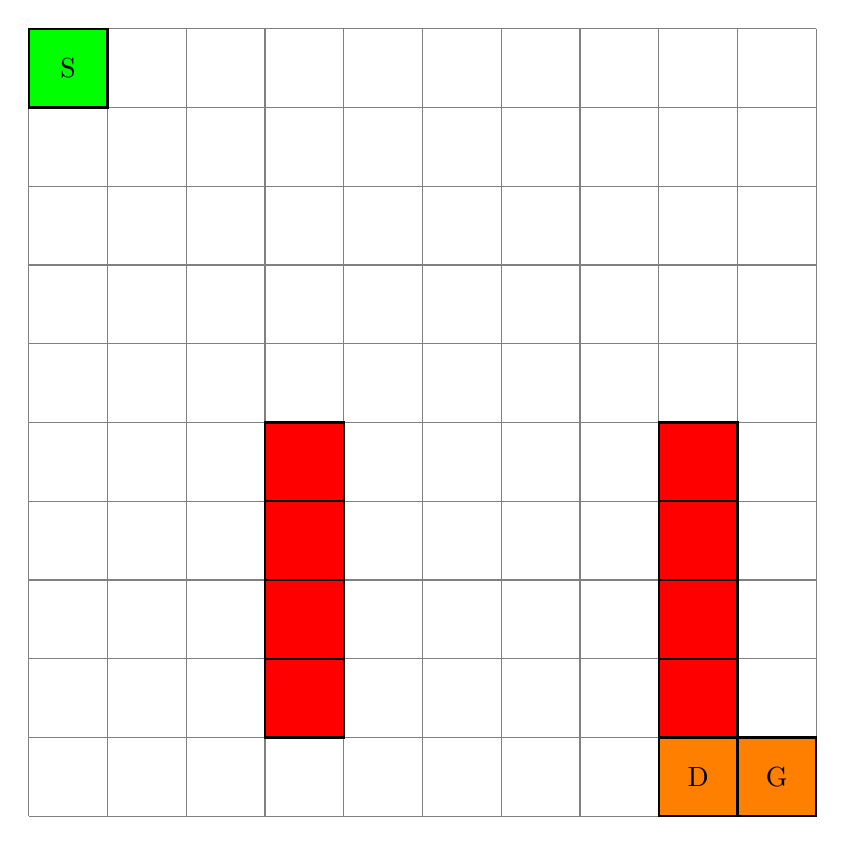
\begin{tikzpicture}
\draw[step=1.0 cm,color=gray] (0,0)grid (10,10);
% col, row
\node[rectangle,draw=black,thick, minimum size=1cm, fill=green] at (.5,9.5) {S};
\node[rectangle,draw=black,thick, minimum size=1cm, fill=red] at (3.5,1.5) {};
\node[rectangle,draw=black,thick, minimum size=1cm, fill=red] at (3.5,2.5) {};
\node[rectangle,draw=black,thick, minimum size=1cm, fill=red] at (3.5,3.5) {};
\node[rectangle,draw=black,thick, minimum size=1cm, fill=red] at (3.5,4.5) {};
\node[rectangle,draw=black,thick, minimum size=1cm, fill=red] at (8.5,1.5) {};
\node[rectangle,draw=black,thick, minimum size=1cm, fill=red] at (8.5,2.5) {};
\node[rectangle,draw=black,thick, minimum size=1cm, fill=red] at (8.5,3.5) {};
\node[rectangle,draw=black,thick, minimum size=1cm, fill=red] at (8.5,4.5) {};
\node[rectangle,draw=black,thick, minimum size=1cm, fill=orange] at (9.5,.5) {G};
\node[rectangle,draw=black,thick, minimum size=1cm, fill=orange] at (8.5,.5) {D};
\end{tikzpicture}
\end{center}
\caption{Medical Domain 2 Grid World}
\label{fig:gridworld2}
\end{figure}
